%%%%%%%%%%%%%%%%%%%%%%% file template.tex %%%%%%%%%%%%%%%%%%%%%%%%%
%
% This is a general template file for the LaTeX package SVJour3
% for Springer journals.          Springer Heidelberg 2010/09/16
%
% Copy it to a new file with a new name and use it as the basis
% for your article. Delete % signs as needed.
%
% This template includes a few options for different layouts and
% content for various journals. Please consult a previous issue of
% your journal as needed.
%
%%%%%%%%%%%%%%%%%%%%%%%%%%%%%%%%%%%%%%%%%%%%%%%%%%%%%%%%%%%%%%%%%%%
\documentclass[twocolumn]{svjour3}      
\smartqed
\usepackage{graphicx}
\usepackage{tikz}
\usepackage{pgfplots}
\usepackage{color}

\pgfplotscreateplotcyclelist{color}{%
    blue,every mark/.append style={fill=blue!80!black},mark=*\\%
    red,every mark/.append style={fill=red!80!black},mark=square*\\%
    brown!60!black,every mark/.append style={fill=brown!80!black},mark=otimes*\\%
    black,mark=star\\%
    red!70!white,mark=star\\%
    lime!80!black,every mark/.append style={fill=lime},mark=diamond*\\%
    cyan!60!black,every mark/.append style={fill=cyan!80!black},mark=otimes*\\%
    yellow!60!black,densely dashed,
        every mark/.append style={solid,fill=yellow!80!black},mark=square*\\%
    black,every mark/.append style={solid,fill=gray},mark=otimes*\\%
    blue,densely dashed,mark=star,every mark/.append style=solid\\%
    red,densely dashed,every mark/.append style={solid,fill=red!80!black},mark=diamond*\\%
}

\pgfplotscreateplotcyclelist{color2}{%
    blue,every mark/.append style={fill=blue!80!black},mark=*\\%
    red,every mark/.append style={fill=red!80!black},mark=square*\\%
    black,mark=star\\%
    lime!80!black,every mark/.append style={fill=lime},mark=diamond*\\%
    yellow!60!black,densely dashed,
        every mark/.append style={solid,fill=yellow!80!black},mark=square*\\%
}

\begin{document}

%Applying List Scheduling Algorithms In A Multithreaded Execution Environment
\title{Aproximating Static List Schedules in Dynamic Multithreaded Applications\thanks{This work is part of the project ``Green Grid'', supported by PRONEX FAPERGS/CNPq and PqG (11/1065-1) FAPERGS grants.}}
%\subtitle{Do you have a subtitle?\\ If so, write it here}

%\titlerunning{Short form of title}        % if too long for running head

\author{Cícero A. S. Camargo\thanks{Supported by grant CAPES (\emph{Coordenadoria de Aperfeiçoamento de Pessoal de Nível Superior}.}\and
        Gerson G. H. Cavalheiro
        \and Maurício L. Pilla
        \and Simone A. da Costa
        \and Luciana Foss
}

%\authorrunning{Short form of author list} % if too long for running head

\institute{Federal University of Pelotas (Brazil)\at
              Gomes Carneiro, 1 \\
              Tel.: +55 53 3921-1327\\
              \email{\{cadscamargo,gerson.cavalheiro\}@inf.ufpel.edu.br \\
			  \{pilla,simone.costa,lfoss\}@inf.ufpel.edu.br}
}

%
\date{Received: date / Accepted: date}
% The correct dates will be entered by the editor


\maketitle

\begin{abstract}

List scheduling algorithms are known to be efficient when the application to be executed can be described statically as a directed acyclic graph (DAG) of tasks. Regardless of knowing the entire DAG beforehand, obtaining an optimal scheduling in a parallel machine is a NP-hard problem. Moreover, many programming tools propose the use of scheduling techniques based on list strategies. This paper presents an analysis of scheduling algorithms for multithread programs in a dynamic scenario where threads are created and destroyed during execution. We introduce an algorithm to convert DAGs describing applications as tasks into directed cyclic graphs (DCGs) describing the same application designed in a multithreaded programming interface. Our algorithm cover case studies described in previous works, successfully mapping from the abstract level of graphs to the application environment. These mappings preserve the guarantees offered by the abstract model, providing efficient scheduling of dynamic programs that follow the intended multithread model. We conclude the paper presenting some performance results we obtained by list schedulers in dynamic multithreaded environments and we compare these results with the best scheduling we could obtain with similar static schedulers.

\keywords{List Scheduling, Multithread Environment, Dynamic Execution}

\end{abstract}

\section{Introduction}

With the increasing popularization of multicore processors, parallel programming has almost become obligatory in the development of any kind of software. Parallel computers, that were once found only in academic or high-performance computing environments, are now ubiquitous. The rise on the demand for programmers that are capable of understanding the issues of these architectures is a direct consequence of this shift from sequential to parallel programming. However, migration to parallel programming paradigms is not simple, as they require a larger abstraction effort. The predicted increase on the number of cores to tens or hundreds of cores per chip will further increase programming complexity.

One way to decrease programming complexity is by providing an efficient scheduling at runtime, so that the programmer just needs to describe the concurrency of the application regardless of the underlying hardware. Nevertheless, obtaining optimals schedules is a NP-hard problem~\cite{casavant88}, and such class of scheduling strategies can be applied only to static problems -- where the structure of the parallel program, as well as the parallel hardware, are known {\em a priori}. Even considering these restrictions, the abstraction of scheduling is successfully employed by many comercial programming tools such as OpenMP~\cite{ChandraOpenMP} and Intel\textregistered~Threading Building Blocks~\cite{TBB2007}, and many academic and research programming tools, such as Cilk~\cite{Cilk95} and Athreads~\cite{VecParLNCS}.

In this paper we evaluate the performance of greedy scheduling techniques~\cite{ListScheduling1989,ListScheduling1990} as the runtime support for dynamic multithreaded programs. Our focus is a scheduling technique that employs a heuristic to determine which thread in a multithreaded program is executing tasks in the \emph{critical path}. This approach has been explored by different academic and research high performance computing runtime environments, such as Cilk~\cite{Cilk95}, and Anahy~\cite{VecParLNCS}. Although case studies and empyric evaluation of these environments have shown satisfactory performance, there are no works that compare the performance of static and dynamic schedulings for the same applications. 

This work recovers results presented by Graham~\cite{Graham76}, then map the case studies to an abstraction of program developed in a multithread programming interface, comparing Graham's static schedules with a dynamic schedule for the mutithread abstraction. The main issue that arises is how to compare the schedule of an application described as a DAG of tasks, the required input for list algorithms, against the schedule of the same application described in a cyclic graph of threads (DCG), this later schedule being obtained by the execution of the DCG in a multithreaded dynamic environment.

In this work, Anahy is the chosen multithread programming interface. Thus we present a set of patterns that allow us to transform a DAG abstraction into a graph representing the control flow of an Anahy program. The we present a dynamic scheduling strategy based on List algorithm to schedule a multithreaded program on a hypothetical architecture, and we finally show the performance obtained by applying this strategy to multithread programs. We can then compare, for a given application, the performance obtained by our dynamic scheduling with the performance resulted by applying static strategies. The results indicate that, for the case studies evaluated, a greedy heuristic can be as good in a multithread dynamic environment as List algorithm can in a static scenario for a given application. However, the programmer should be aware of the environment's scheduling strategy and manage the dependencies between threads to take advantage of this.

This work is an extension of the one published in~\cite{CiceroHPCLatam2012}. In this extension we discuss the approximation of static list scheduling algorithms in dynamic multithreaded environments and then present scheduling results obtained in several simulations as well as executions in real multithreaded environments.

The remainder of the paper is organized as follows. List scheduling and critical path heuristic are described in Section~\ref{sec:listscheduling}. Section~\ref{sec:proginter} presents a model for a multithreaded programming interface. The process of a creation of a DCG from a DAG is described in Section~\ref{sec:DAG2DCG}, and in Section~\ref{sec:evaluation} performance of static and dynamic scheduling are compared. Section~\ref{sec:practical_results} presents case studies of applying list scheduling strategies in dynamic multithreaded environments, where one of these cases shows actual execution in real multithreaded environments. Finally,  Section~\ref{sec:conclusion} presents the concluding remarks.

\section{List Scheduling Algorithms} \label{sec:listscheduling}

List scheduling algorithms receive a Directed Acyclic Graph~(DAG) as input and produce a schedule over $m$ available processors. The input DAG describes a parallel program in terms of tasks (represented by nodes) and their dependencies (represented by directed edges). As an online technique, list scheduling algorithms do not analyze the nodes that follow a task to decide the current scheduling, since these tasks could not be present in the DAG at runtime. Furthermore, heuristics can be applied to determine priority rules for the tasks allowing the scheduler to select the most suitable one to optimize some performance index.

The following subsections define the basic structure of dataflow programs, what is a direct acyclic graph, and the basic greedy scheduling algorithm. 

\subsection{A Dataflow Program}

Programs describing their tasks in terms of data dependences are suitable to be described in a DAG. In the dataflow model~\cite{dataflowAdvances2004}, a task consists of a sequence of instructions between two synchronization points: the input and the output of data. Any other synchronization mechanism is not allowed. Tasks can be represented as functions $y= f(x)$, $x$ and $y$ representing the input and output set of data. A given task is said to be ready to execute when its input operands become available. When $f$ is finished, its output values may then be taken as input by other tasks. 

This execution model is very attractive for several reasons~\cite{prasanna2005}, such as:  {\em (i)}~tasks use data items defined in a higher level of abstraction without worrying about how they are produced, and {\em (ii)}~programs are highly extensible and reusable because there is no direct task-to-task coupling. Another aspect is its original research motivation in the context of the exploitation of massive parallelism~\cite{dataflowAdvances2004}.

\subsection{Directed Acyclic Graph}

A \emph{Directed Acyclic Graph}~(DAG) is a representation of an application in terms of tasks and dependencies between tasks. The nodes in the graph represent the tasks and the directed edges represent the input/output data of these tasks. Nodes may be weighted with their computational costs, while edges may be weighted with communication costs. A more formal description of a DAG follows: 

\begin{definition}
A DAG is a tuple $G = (V, A) $ representing a program $P$. In this tuple, $V$ corresponds to the set $n$ of nodes and $A$ to the set of edges in $G$. Each node in $V$ receives a label~$i$, where $1 \le i \le n$, in order to represent the task $\tau_i$ in the graph: $V = \{\tau_1, \tau_2, … \tau_n\}$.
A precedence relation between $\tau_i$ and $\tau_j$ is represented by $\tau_i \prec \tau_j$ and defines a direct edge in the graph: $A = \{(\tau_i \prec \tau_j) | 1 \le i,j \le n, i \neq j\}$. If the program $P$ describes that $\tau_i$ is an immediate predecessor of $\tau_j$, then $(\tau_i \prec \tau_j) \in A$. Such dependence means that $\tau_j$ cannot be started before $\tau_i$ has been finished, because the output of $\tau_i$ must be available to $\tau_j$ so it can be started.
In this representation, nodes and edges are weighted: $|\tau_i|$ and $|\tau_i \prec \tau_j|$ correspond to the computational cost associated to $\tau_i$ and to the data transfer cost associated to $\tau_i \prec \tau_j$, respectively. 
\end{definition}

From the previous definition we assume that $G$ can have transitive edges: if $\tau_i$, $\tau_j$ and $\tau_k$ are tasks defined by the application and $\tau_i \prec \tau_j$, $\tau_i \prec \tau_k$ and $\tau_j \prec \tau_k$ are precedence constraints in this application, $(\tau_i$, $\tau_j$, $\tau_k$) $\in V$ as well as $(\tau_i \prec \tau_j$), ($\tau_i \prec \tau_k$), ($\tau_j \prec \tau_k) \in A$.

The input tasks and the output tasks can also be identified, that is, the tasks that are ready to execute when the program is launched and the tasks that do not produce data to any other task in the program. Input tasks are the subset $V^{in}$ of tasks $\tau_i$ whereas there is not $(\tau_j \prec \tau_i) \in A$. Output tasks are the subset $V^{out}$ of tasks $\tau_i$ whereas there is not $(\tau_i \prec \tau_j) \in A$.

\subsection{Priority Attributes}
\label{sub:priority_attributes}

Whenever two or more executable tasks contend for a free processor, the selection of the right task is done by their priority of execution, which is set according to some strategy. If there is more than one task ready with the same piority, ties can be broken randomly.

Considering the length of a directed path in the graph as the sum of the weights of all vertices and edges along the path including the initial and final vertices, we can define two major priority attributes found in the literature: the \emph{level} (or \emph{bottom-level}), and the \emph{co-level} (or \emph{top-level}). Both are defined in the same sense as in~\cite{coffman1973operating}. The \emph{level} of an output task $\tau_i$ in $G$ is $|\tau_i|$, and the \emph{level} of a non-output task $\tau_i$ is the longest path from $\tau_i$ to an output task. The \emph{co-level} is defined in the same way, but the references are the input tasks. Thus the \emph{co-level} of an input task $\tau_i$ in $G$ is $|\tau_i|$, and the \emph{co-level} of a non-input task $\tau_i$ is the longest path from $|\tau_i|$ to an input task.

Several List Scheduling Algorithms like the following are based on These two attributes.
\begin{itemize}
	\item HLFET (Highest Levels First with Estimated Times): A-Schedules~\cite{coffman1973operating} are list schedules which consider the priority of a task as being its \emph{level};
	\item HLFNET (Highest Levels First with No Estimated Times): This algorithm considers (possibly incorrectly) that all tasks have the same execution time and their priority attibute is their \emph{level}. HLFNET can be used when HFLET is desirable but we can't know tasks execution times in advance.
	\item RANDOM: Task priority values are assigned randomly. Random and optimal schedules are common bases to compare other list schedules.
	\item SCFET (Smallest Co-levels First with Estimated Times): This algorithm considers the priority of a task as the negative of its \emph{co-level}.
	\item SCFNET (Smallest Co-levels First with Estimated Times): This algorithm works the same as SCFET, but all tasks are assumed to have the same execution time.
\end{itemize}

There are applications where the DAG is built dynamically as the program evolves. In these cases we can not use an algorithm like HLFET/HLFNET which needs the entire graph structure, from input to output vertices, to calculate the priority attribute for a task. However, algorithms like RANDOM and SCFET/SCFNET can be used for situations when certain tasks can be inserted in the graph asynchronously or one of its predecessors decides to create it. We can also use the arrival time of tasks to assign priorities during execution time. Two major algorithms are built over this idea: LIFO (Last In, First Out) gives higher priority to the most recently created task; FIFO (First In, First Out) gives higher priority to oldest ready task.

\subsection{A Greedy Scheduling Strategy} \ref{ssec:greedy_strategy}

The purpose of a scheduling $S$ is to complete the execution of a given DAG $G$ in a finite time. Scheduling algorithms usualy include strategies to minimize an index of performance, such as the total execution time, as considered in this paper. We note $|S(G)|$ the length of the scheduling, that is, the time required to complete the execution of all tasks in $G$. The basic list scheduling algorithm runs as follows.

{\small
\begin{itemize}
\item Input: graph $G$ and a set of $m$ identical processors.
\item Output: $|S(G)|$.
\end{itemize}
\begin{enumerate}
\item Set all input tasks in $G$ as \emph{READY} and the remaining as \emph{NOT\_READY}
\item $L = V$
\item Sort($L$)
\item \textbf{EACH} processor $\in m$ \textbf{DO (IN PARALLEL)}
   \begin{enumerate}
		\item $\tau$ = GetReadyTask($L$)
		\item \textbf{IF} $\tau$ is \textbf{NOT} \emph{NULL}
            \begin{enumerate}
              \item Run $\tau$
              \item Set $\tau$ as \emph{FINISHED}
			  \item Update $\tau$'s successors
            \end{enumerate}
		\item \textbf{END IF}
   \end{enumerate}
\item \textbf{UNTIL} $\tau$ is \emph{NULL}
\end{enumerate}
}

This basic strategy makes several assumptions: \emph{(i)} a set of $m$ processors is responsible for executing the \emph{for each} loop concurrently, running the tasks described in $G$; \emph{ii} Sort($L$) is an algorithm like the ones described in Section~\ref{sub:priority_attributes}, that sorts the list of vertices $L$ in decreasing order of priority; \emph{(iii)} GetReadyTask($L$) always returns a valid task, unless the graph's computation is completed; if not NULL, the task's state is atomically set to RUNNING before the function returns; if there are not \emph{READY} tasks at the moment, the function blocks the applying processor until some task becomes READY; \emph{(iv)} lines labeled as \emph{ii} and \emph{iii} are executed atomically. 

This basic strategy was studied in several papers. Graham~\cite{Graham66} defines the concept of Critical Path to give the priority to each task and analyzes the  worst-case performance. A Critical Path~$CP$ is a subset of $V$ that contains the tasks present in the longest sequence of dependences. The concept of a critical path allows the estimation of upper and lower bounds for the time $T_m$ required to schedule a graph $G$ in a machine with $m$ identical processors.
Considering that there are no scheduling and communication costs, the constraints for time $T_m$ are defined as~\cite{Graham66}: 

	\begin{equation}
	\frac{T_1}{m} \le T_m \le \frac{T_1}{m} + T_\infty
	\end{equation}

\noindent where:
\begin{itemize}
  \item  $T_{1} = \sum_{i=0}^{n} |\tau_{i}| , \forall   \tau_{i} \in V$, that is, the sum of all computational costs of tasks in $G$.
\item $T_{\infty} = \sum_{i=0}^{k} |\tau_{i}| ,  \forall   \tau_{i} \in CP$, that is, the sum of all computational costs of tasks present in the Critical Path of $G$. 
\end{itemize}

Since the tasks in a Critical Path must be executed in sequence, the sum of the computational cost in this path represents the minimum execution time expected for the application, independent from the number of available processors. Graham~\cite{Graham76}  presents several case studies involving the scheduling of DAGs. Further works like~\cite{bartal95,karger96,Albers99,Fleischer2000} extend the results of Graham's.

\section{Multithreaded Programming Model}\label{sec:proginter}

The multithreaded programming model is employed to write parallel programs in terms of concurrent execution flows sharing a common memory address space. The interface facilities of this program must include primitives to create and synchronize execution flows and to guarantee safe accesses to shared data. We discuss in this section an abstraction of this model to create a Directed Cyclic Graph to represent the control flow among threads.

\subsection{Evolving a multithread program}

In a multithreaded program, each thread is responsible for executing a specific sequence of instructions. The final result is an arrangement of the partial results computed by each thread. We assume that threads can be dynamically created and destroyed during the execution of a program by invocating a specific service.

Communication among threads may be implemented in two ways, both of them considering that the data itself is present in a shared addressing space. The first method explores the explicit synchronization introduced by invocations to create and join primitives. By monitoring calls to those primitives it is possible to guarantee the control of the execution flow in order to establish a deterministic behavior for the program. 
A second strategy is to employ semaphores, or other equivalent constructors, to control the execution of threads in a mutual exclusion mode when accessing data in the shared addressing space. A drawback of this strategy is that it is impossible to guarantee an execution order among threads and the execution will be, necessarily, nondeterministic.

\subsection{Directed Cyclic Graph}

In the present work, a restriction to the communication among threads is imposed: threads may not employ mutual exclusion synchronization mechanisms. Our programming model allows communication among threads at creation or termination time.
Hence, these restricted threads become similar to the definition of a task: a thread can be represented as a function $y = F(x)$, since there is no collateral effects in global data. In the same way as in the task model, when $F$ is finished its output values can be received by other threads but differently of the task model, a thread is said to be ready to execute just after its creation, since its input parameters are received during the creation process. Another important difference from tasks is that the code of a thread may include instructions to fork (\emph{create}) new threads or to wait for the end of other threads (\emph{join}). Therefore, a graph generated by a multithreaded execution is said to be directed with cycles (DCG – {\em Directed Cyclic Graph}).

\begin{definition}
A DCG is a tuple $C = (N, E) $ representing a program $P$. In this tuple, $N$ corresponds to the set $n$ of nodes and $E$ to the set of edges in $C$.
Each node in $N$ receives a label $i$, where $1 \le i \le n$, in order to represent the thread $\Gamma_i$ in the graph: $N = \{\Gamma_1, \Gamma_2, … \Gamma_n\}$.
A precedence order among instructions of two threads $\Gamma_i$ and $\Gamma_j$ is represented by $\Gamma_i \rightarrow \Gamma_j$, in the graph: $E = \{\Gamma_i \rightarrow \Gamma_j | 1 \le i,j \le n, i \neq j\}$.
There is a directed edge from $\Gamma_i$ to $\Gamma_j$ if the program $P$ describes that $\Gamma_i$ creates $\Gamma_j$ or that $\Gamma_j$ synchronizes with the termination of $\Gamma_i$. That means that or $\Gamma_j$ can be started just after it has been created by $\Gamma_i$ either that $\Gamma_j$ must remains blocked until to be guaranteed that $\Gamma_i$ has finished.
In this representation nodes and edges are weighted: $|\Gamma_i|$ and $|\Gamma_i \rightarrow \Gamma_j|$ correspond to the computational cost associated to $\Gamma_i$ and to the data transfer cost associated to $\Gamma_i \rightarrow \Gamma_j$, respectively.
\end{definition}

From the definition of a DCG it is allowed to have both $\Gamma_i \rightarrow \Gamma_j$ and $\Gamma_i \rightarrow \Gamma_k$, represented by $\Gamma_i \rightarrow \Gamma_{j,k}$ as well as $\Gamma_i \rightarrow \Gamma_j$ and $\Gamma_k \rightarrow \Gamma_j$, represented by $\Gamma_{i,k} \rightarrow \Gamma_j$. The first case ($\Gamma_i \rightarrow \Gamma_{j,k}$) represents a split (multiple thread creation) operation and the second one a reduce (merge of multiple threads) operation.

Another characteristic inherent to the practice of multithread program is that the execution begins by the execution of one thread (the thread $\Gamma_1$) and finishes executing only one thread (the same $\Gamma_1$).

\subsection{Scheduling threads at application level}

There are many strategies to schedule threads at user level, such as the ones implemented in OpenMP~\cite{ChandraOpenMP}, Athreads~\cite{Vicosa07}, and Cilk~\cite{Cilk95}.

In OpenMP user level threads are created in a nested fork-join structure. The runtime scheduler distributes the work generated among the processors. Three strategies are available to distribute the threads: \emph{cyclic}, \emph{dynamic}, and \emph{guided}. The first one sends equal amounts of work to each processor. The \emph{dynamic} and \emph{guided} strategies can be used to adjust the load distribution in function of the difference of loads among the threads. Such a programming interface is very attractive when the application may be described in terms of data parallelism.

The Cilk programming interface provides two synchronization primitives: {\em spawn} to create a thread and {\em sync} to synchronize at once all threads created by the current thread in a nested fork-join structure. There is no explicit data exchage among threads, those synchronization primitives indicate that a set of data are ready to be read from a shared addressing space. The Cilk runtime builds a graph describing the dependences among threads. This graph is handled by the scheduler in order to distribute the load among the processors and to control the execution order. The scheduler algorithm is implemented in two layers known as \emph{work stealing}~\cite{blumofe1994scheduling}. At local level, running on each processor, the deeper a thread is in the subsection of the graph handled by the processor, the higher is its priority. At global level, threads can migrate from a processor to another when a processor becomes idle and choses a victim processor to steal work from. In this case, the higher a thread is in the graph, the higher is its priority to be stolen.

Athreads is an implementation of Anahy~\cite{VecParLNCS} model. Its programming interface proposes two primitives to handle threads and to communicate data among them: {\em create} and {\em join}. These primitives allow the creation or synchronization of $n \geq 1$ threads at once, like split or reduce operations -- the runtime implements a kind of garbage collector to check references to finished threads. Addresses of data in a shared dynamic heap are passed to threads at creation time, and also as return values when a thread terminates. Athreads' runtime also generates a graph representing the control flow in reaction to the execution of create/join services but the generated graph is unstructured.  
From this graph, it is possible to extract a tree representing the creation of threads: each thread represents the root of a subtree, and its children are all threads it has created. When a processor becomes idle, the higher branch of the tree, i. e., the thread containing the oldest ready task not yet executed, is selected by the scheduler. Locally to the processor, the closer a thread is to the root of the subtree, the higher is the priority.

\section{Building a DCG from a DAG}\label{sec:DAG2DCG}

List Scheduling strategies are the basis of both Cilk and Athread runtime. More specifically, a List strategy which takes into account the Critical Path. In both environments the heuristic applied is that the Critical Path starts and finishes in the first and last tasks of the first launched thread. Both environments handle threads at application level, and empirical results~\cite{Cilk95,VecParLNCS} show that they achieve good performance for some kinds of applications. In the present work we are interested in evaluating how far the performance obtained by dynamic list schedules that take a DCG as input is from static DAG schedules.

\subsection{Preliminaries and methodology}

The first study of List Scheduling was presented in 1966 by Graham~\cite{Graham66}. He has shown that the online greedy algorithm can change the schedule length by a factor of at most $2 - \frac{1}{m}$ depending on the order of task arrival. The model introduced by Graham considers that the scheduling does not incurs in any overhead and that there are no communication costs. In~\cite{Graham76}, Graham presented a sequence of examples of DAGs being scheduled by List Scheduling, and showed several schedules for them, including the best possible ones. This basic strategy was successfully employed by different multithreaded programming environments, such as Cilk~\cite{Cilk95} and Athreads~\cite{cordeiro2005}, although these programming tools employ DCGs instead of DAGs to represent the control flow.

In this paper, we propose the application of list scheduling to a multithreaded program during runtime. For each DAG presented in~\cite{Graham76}, an equivalent transformation to a DCG is proposed, and the result is submitted to a list scheduling strategy to obtain the scheduling length. Athreads was chosen as the programming interface since it provides resources to build an unstructured graph and both the creation and the synchronizations of multiples threads at once.

The resulting DCGs highlight the control flow among threads but, internally to threads, the tasks of the original DAGs are still represented as well as the original dependencies are still respected.

In the following of this section, we present the translations rules applied to build a DCG from a DAG. Next section presents the case studies and the performance we have obtained.

\subsection{Building Rules}

\begin{figure*}[htb]
\begin{center}
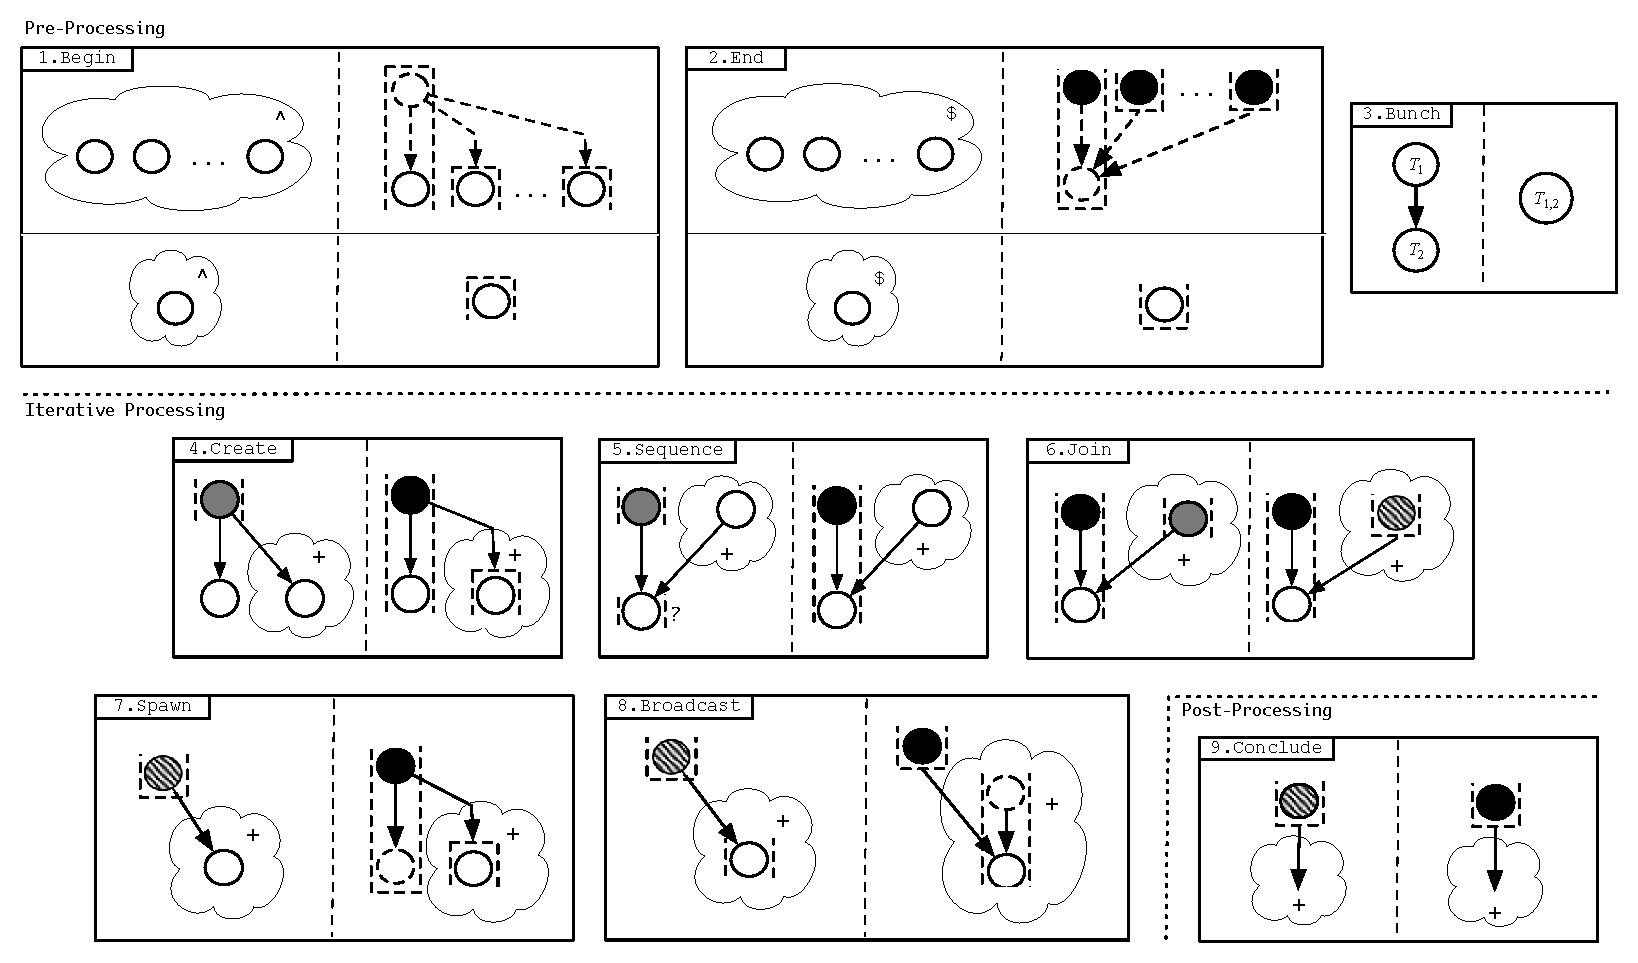
\includegraphics[width=0.9\textwidth,angle=0]{figs/shapes_definitivo.eps}
\caption{Patterns in a DAG and the corresponding segment in a DCG.}
\label{fig:shapes}
\end{center}
\end{figure*}

The creation of a DCG $C_i = (N_i,E_i)$ representing a DAG $G_i = (V_i,A_i)$ preserves the original structure of $G_i$. The creation process consists in encapsulating a sequence of $n \le 1$ tasks of the original $G_i$ in the context of $C_i$ threads. The directed edges between tasks in $G_i$ are preserved in $C_i$, but only the edges representing dependencies between tasks in different threads are included in $E_i$. Those edges represent the creation or the synchronization of threads.

From here on we are going to use extensivelly the term ``left most'', which reflects the way we organize our drawings. By ``left most'' we mean either the task $\tau_i$ with the smallest identifier $i$, when we refer to tasks at the same level in the graph, or threads that are closer to $\Gamma_i$ and were created first in a dynamic multithreaded execution.

In Fig. \ref{fig:shapes} we present a set of nine patterns of relationships among tasks present in a DAG $G_i$ and the rule to be applied to introduce the corresponding section in the DCG $C_i$. In this figure, circles represent tasks in $V_i$, and the dotted rectangles threads in $N_i$. On each pattern, the grey task is the one being evaluated. A hachured task has at least one left most dependence that was already evaluated. An entirely evaluated task is represented in black. Dotted circles are tasks called {\em conforming tasks} ($CT$). Those tasks are introduced to guarantee that the tasks present in $C_i$ will finish executing just one synchronization in order to correspond to the task model adopted by Athreads. In this work we consider $ |\tau^{CT}| = 0 $. A cloud with a $+$ signal involving a thread or a task indicates the presence of at least one of those thread or task.
A symbol $?$ indicates that the element associated can be or not present and the symbols \^~and $\$$ indicate the begin and the end of $G$.

\subsubsection{Preprocessing $G_i$}

The creation process starts by applying the preprocessing patterns. This first pattern, named \verb+Begin+, identifies the tasks in $G_i$ that have no precedence constraints. A conforming task is created to represent the begining of execution and a multiple thread creation. The result of the application of this pattern is that each task with no precedence constraints will represent the first task to be executed in the context of a thread in $C_i$. If there is just one task without precedence in $V_i$, just one thread is added to $N_i$. Notice that the conforming task is introduced in the left most thread since the first thread launched by the program (that is, the {\em main} thread) will be represented in the left most side of $C_i$.

The second pattern, named \verb+End+, identifies tasks without successors in $G_i$. Similarly to the \verb+Begin+, all tasks become the last task to be executed in the context of a thread and a conforming task is added to the leftmost thread to represent the multiple join. In the case were there is just one exit task in $G_i$, just one thread is added to $C_i$. 

The last preprocessing pattern is the \verb+Bunch+, which represents that $(\tau_j \prec \tau_k) \in A_i $ but neither $(\tau_x \prec \tau_k), \forall x \neq j \in A_i $ or  $(\tau_j \prec \tau_x), \forall x \neq k \in A_i $. The resulting $\tau_{j,k}$ cost is $|\tau_{j,k}| = |\tau_j| + |\tau_k|$.

\subsubsection{Iterative processing}

After the preparation of $G_i$, all task in $V_i$ must be visited to identify matching patterns. A task can match one of the following patterns: \verb+Create+, \verb+Sequence+, \verb+Join+, \verb+Spawn+, or \verb+Broadcast+. The tasks in $G_i$ are visited in a breadth-first strategy, taken each level from left to right. If a task matches more than one pattern, the leftmost dependence must be solved first.

The \verb+Create+ and \verb+Join+ patterns correspond to the creation or synchronization of threads. At creation, new threads are added to $C_i$ and the task which succeeds the evaluated task becomes part of the same thread. The \verb+Join+ pattern identifies the termination of threads and the respective synchronization. As result, the thread containing the evaluated task is closed. The \verb+Sequence+ pattern enrolls a task in the context of an existing thread or merges two segments of threads.

Despite the end of a thread being identified, the last task executed by this thread may have other dependences \verb+Spawn+ and/or \verb+Broadcast+. A spawn corresponds to creation of new threads; a conforming task is necessary to express the already evaluated dependencies. A broadcast corresponds to the synchronization of the end of the current thread with others. In this case, two conforming tasks must be inserted in order to guarantee the existing precedence constraints.

\subsubsection{Post-processing $C_i$}

Once all tasks on $G_i$ have been evaluated and introduced in the context of threads on $C_i$, there are no more dependencies to be evaluated. The pattern \verb+Conclude+ identifies the tasks which have matched the pattern \verb+Join+ without being followed by any other dependence.

Since the nodes of the graph are visited in a breadth-first strategy and that left dependencies are evaluated first, a larger amount of work is expected to be present in the left side of the DCG. A scheduling heuristic can be applied to explore the presence of the Critical Path in the left most threads.

\section{Appling List Scheduling to DCGs}\label{sec:evaluation}

In this section we evaluate the use of a simple scheduling algorithm based in a List Strategy introduced in the runtime of a multithread environment. We present this algorithm and we compare its performance with one presented by the original Graham scheduling. 

\subsection{Basic List Scheduling Strategy}\label{sec:schedalgo}

The proposed scheduling strategy takes as input a DCG $C = (N,E)$ to be executed in a parallel architecture $P = (P_1, P_2, \dots P_m)$ with $m$ homogeneous processors. The graph is built at execution time: a thread creation introduces new nodes in the DCG and new edges from the node hosting the current thread to the new ones as well as a join adds a new edge from the node(s) representing the thread(s) to be synchronized with the node hosting the thread asking for synchronization. The scheduler can mark nodes in $C$ to identify the current status of the thread.

The scheduler runs as follows in a parallel machine with $m$ identical processors. The first thread on the application ($\Gamma_1$) becomes the first node in of the DCG and is annotated as {\em ready}. In this graph, closer a {\em ready} thread is from the root node, higher is its priority to be chosen when a processor becomes idle. When a processor $P_i$ becomes idle it takes from the graph a node and marks the corresponding thread as {\em executing}. Once a thread is finished, the corresponding node is marked as {\em terminated} and the processor becomes idle. During its execution, a thread may request join operation. In this case, the synchronized threads can be marked as {\em terminate}, {\em ready} or {\em executing}. In the first situation, the current thread can continue its execution. If the synchronized thread is {\em ready}, the scheduler suspends the execution of the current thread and launch over this processor the synchronized thread. In the last situation, the synchronized thread is {\em executing}, the scheduler also suspends the execution of the current thread and chose another one to be launched in the portion of the graph having the synchronized thread as root; this processes is repeated as many time as necessary. The execution of a thread is resumed when its synchronization requirement is satisfied.

\subsection{Building DCGs}

\begin{figure*}[htb]
\begin{center}
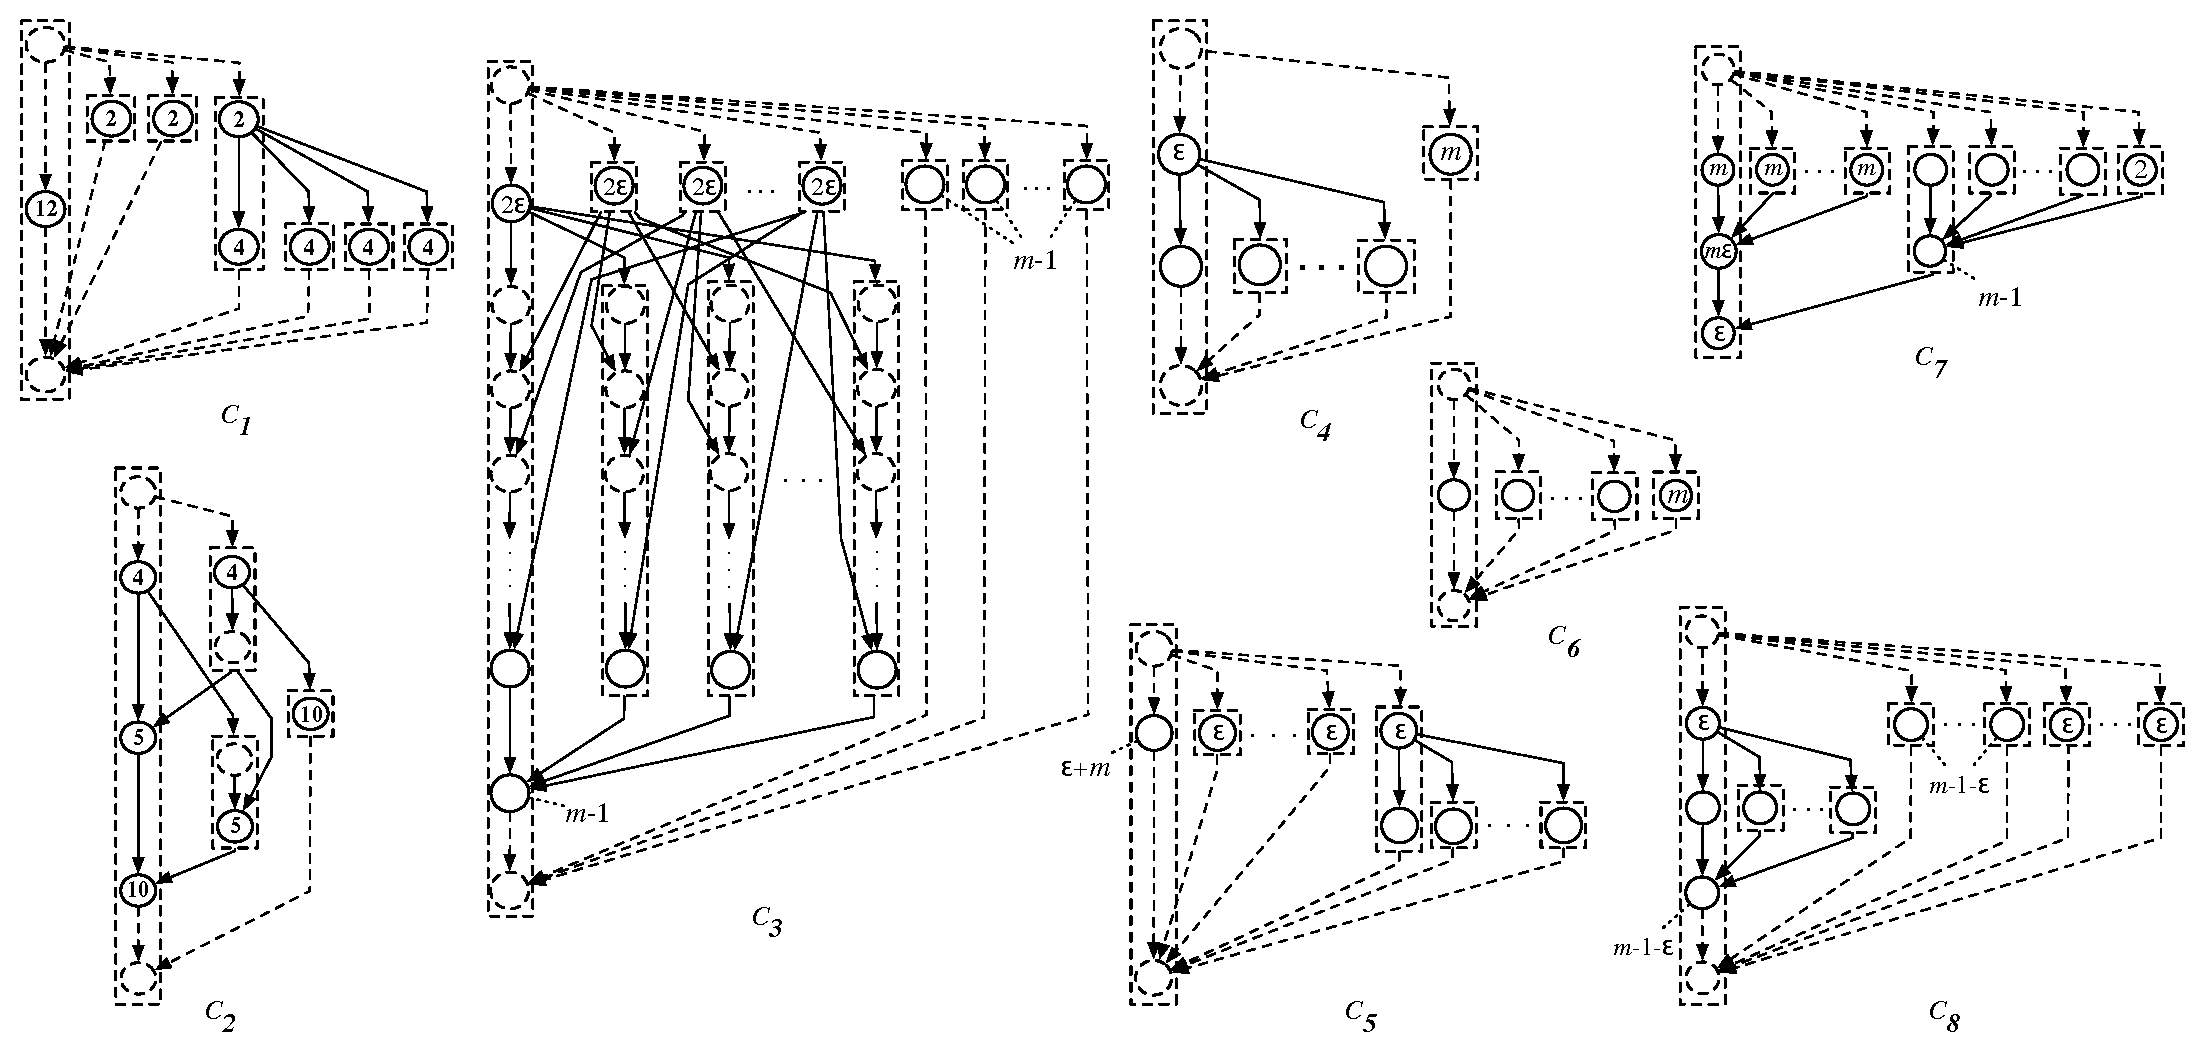
\includegraphics[width=1.0\textwidth,angle=0]{figs/transformacoes.eps}
\caption{Result of the application of DCG generation.}
\label{fig:dgcdograham}
\end{center}
\end{figure*}

Our case study are the examples 1, 2, 4, 5, 6, 7, 9 and 10 presented in \cite{Graham76}. We name those graphs as $G_1, G_2, \dots G_8$ and we present in Fig. \ref{fig:dgcdograham} the corresponding $C_i$, obtained by applying the proposed process. The number at the interior of each task represents its computational cost – this cost can be presented in terms of the number $m$ of available processors or in terms of $\varepsilon$, representing a very small cost, if none, the cost is~1. The conforming tasks have cost 0~(zero).

\subsection{Scheduling the Case Studies}

The performance of our case study is presented in terms of scheduling length, i.e., the time required to execute the corresponding application. Table \ref{tab:resultados} presents those execution times. The first two columns represent the corresponding input graph ($C_i$/$G_i$) in Fig.~\ref{fig:dgcdograham} and the number $m$ of available processors. The third column present the execution time $|S(C_i)|$ obtained with our scheduling. The fourth colunm presents the best scheduling $|S(G_i)|$ obtained for a given DAG and the fifth column is the scheduling $|S'(G_i)|$ obtained for the same DAG changing the priority list. The last column will be explained later.

\begin{table*}
\begin{center}
\caption{Scheduling of $C_i$.}\label{tab:resultados}
\begin{tabular}{c|c||c||c|c||c}
DCG/DAG & \# $m$ & $|S(C_i)|$ & $|S(G_i)|$ & $|S'(G_i)|$ & $|S(C_i')|$\\ \hline\hline
$C_1$/$G_1$ &  3  & 12 & 12 & 14 & --\\ \hline
$C_2$/$G_2$ &  2  & 19 & 19 & -- & --\\ \hline
$C_3$/$G_3$ & $m$ & $2m-1+2\varepsilon$ & $m+2\varepsilon$ & -- & $m+2\varepsilon$ \\ \hline
$C_4$/$G_4$ & $m$ & $m+\varepsilon$ & $m+\varepsilon$ & -- & --\\ \hline
$C_5$/$G_5$ & $m$ & $m'+2\varepsilon$ & $m'+2\varepsilon$  & -- & --\\ \hline
$C_6$/$G_6$ & $m$ & $2m-1$ & $m$ & $2m-1$ & $m$\\ \hline
$C_7$/$G_7$ & $m$ & $2m+\varepsilon$ & $(m+1)(1+\varepsilon)$ & $2m+\varepsilon$ & --\\ \hline
$C_8$/$G_8$ & $m$ & $2m-1-2\varepsilon$ & $m$ & $2m-1-2\varepsilon$ & --\\ \hline
\end{tabular}
\end{center}
\end{table*}

Since our scheduling strategies give higher priority to threads in the left side of $C_i$, supposing that the Critical Path will be present in this side of the DCG, we compare our results with the best ones obtained by Graham. We observe that our scheduling provides to graphs $C_1$, $C_2$, $C_4$ and $C_5$ the same performance as the best obtained by scheduling the corresponding DAG. In another hand, the performance of our strategy is not optimal for the graphs $C_3$, $C_6$, $C_7$ and $C_8$.

The algorithm converts a DAG into its equivalent DCG considering the order of the tasks in the input graph as the temporal order of their creation. The mechanism match the patterns in a breadth-first order. This way, the DCG generated does not always take advantage of the scheduling technique used by the execution environment. However, if the programmer is aware of the process of building a DCG and the scheduling algorithm, he can reorganize the DAG without prejudice to the precedence constraints arranging the tasks to fit both. Thus, graphs $G_3$ and $G_6$ can be rewritten to result the DCGs showed in Fig. \ref{fig:newC3C6} with execution times $|S(C_i')|$ presented in Table \ref{tab:resultados}.

The situation observed in graphs $C_7$ and $C_8$ is different from that in $C_3$ and $C_6$. In those cases, $|S(C_7)| = |S'(G_7)|$ and $|S(C_8)| = |S'(G_8)|$ since the scheduler $S'$ corresponds to a strategy based in the Critical Path, the same heuristics applied by our scheduling algorithm. Therefore, our scheduling cannot produce better results, as expected by a tipical greedy list scheduling algorithm.

\begin{figure}[htb]
\begin{center}
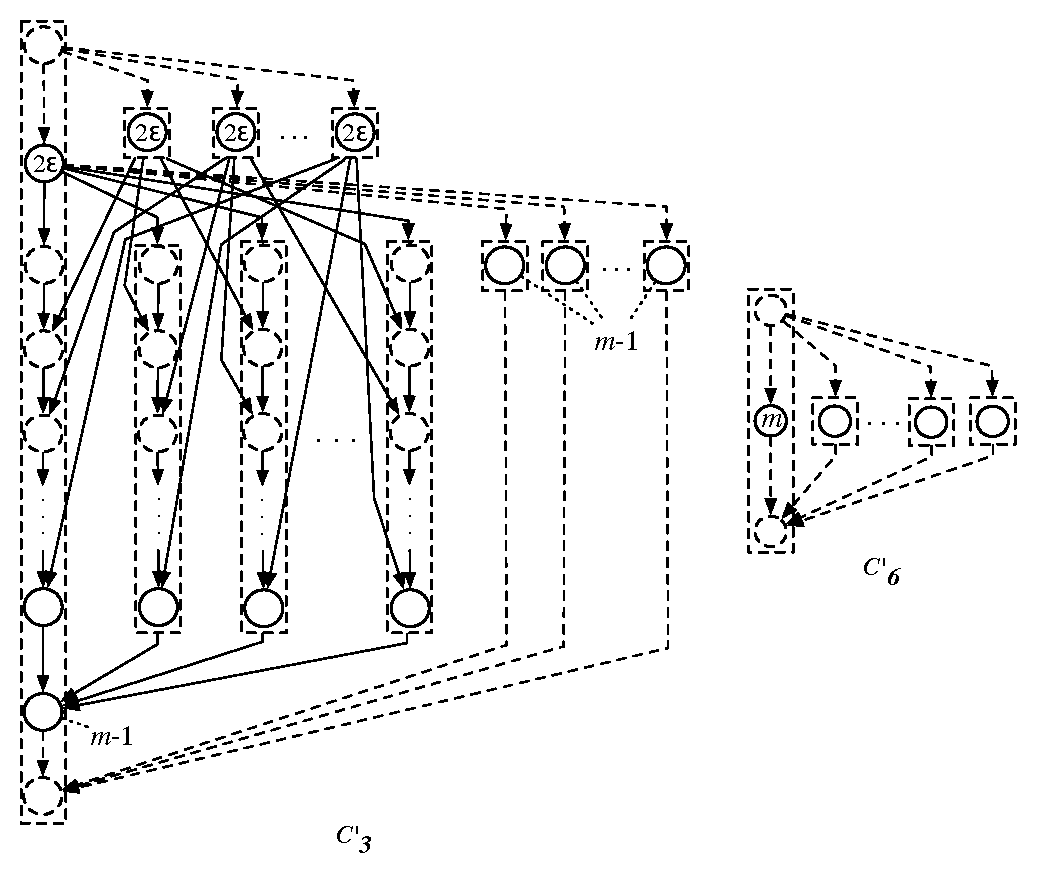
\includegraphics[width=0.5\textwidth,angle=0]{figs/cl3_cl6.eps}
\caption{Transformation over graphs $G_3$ and $G_6$ rewritten to fit the scheduling strategy.}
\label{fig:newC3C6}
\end{center}
\end{figure}

\section{Approximating Static Scheduling} \label{sec:practical_results}

The purpose of this section is to present a study on the performance of different heuristics for prioritizing tasks in dynamic multithreaded environments. This study aims to measure the distance, in terms of the schedule lenght, between dynamic multithread scheduling and static DAG scheduling, both using list algorithms. In the first part of the study we simulated two distinct execution environments, one for programs described in a DAG, the other for programs described in a DCG. We executed several experiments considering five priority policies for each environment. In the second part of the study we implemented the strategy that provided better results in the simulated evironment that cosidered DCGs in the full-fledged multithreaded environment of Anahy. In both parts of the study, we believe that the random strategy for prioritizing tasks is to insert less overhead operations by scheduling no need to select the task / thread to be launched.

\subsection{Simulating Dynamic Scheduling Behavior}

In this Section we will present two case studies to examine the behavior of scheduling a program described in a graph in a simulated dynamic environment using list scheduling algorithms. In both case studies we consider a synthetic application, whose DAG tasks and dependecies are generated ramdomly in a nested fork/join fashion. The cost of each task is measured in terms of time units, and so is the schedule lenght. The results we will show next can only be obtained through simulation, because in a real dynamic execution the DAG is not available \emph{a priori}. So we generate the DAG, obtain the corresponding DCG, and simulate the execution of each program representations over different execution evironments that use list algorithms to do the scheduling. When we simulate the DAG scheduling, the processors run a loop similar to the one presented in the algorithm from Section~\ref{ssec:greedy_strategy}. When we simulate the DCG scheduling, the processors work like described in Section~\ref{sec:schedalgo}, but they can operate in three different execution modes:

\begin{itemize}
\item Work-First (WF): when a processor executes a \emph{create} operation, it starts instantaneously the execution of the newly created thread and the current thread is made available for other processors to resume it, becoming suspended if there is no idle processor. If a processor executes a \emph{join} over a non-finished thread, the current thread remains blocked until the joined thread is finished, when the previously blocked thread can be migrated to any processor to be resumed.
\item Help-First(HF): when a processor executes a \emph{create} operation, the processor continues the execution of the current thread after making the newly created thread available for other processors. During a \emph{join} operation the scenario is the same as in Work-First mode.
\item Help-First without Migration: the processor behaves the same way as in HF during thread creation. However, if a thead gets blocked on a \emph{join} operation only the current processor can resume its execution.
\end{itemize}

For each DAG generated, we scheduled them over the task processors using the algorithms HLFET, HLFNET, RANDOM, SCFET and SCFNET, presented in Section~\ref{sub:priority_attributes}. For each DCG generated, we scheduled them over the thread processors using the algorithms LIFO, FIFO, and RANDOM, and also SCFET and SCFNET, case in wich we bring the priority attributes from task to thread level.

In the first case study we considered that all tasks cost one time unit to be executed. In the second case study each task has a pseudo-random cost inside the interval $[1;10]$. Since for the second case we can have completely different costs for the same graph structure, we run 100 simulations and calculated the average of the results (the standard deviation was always below 5\%).

The schedule lengths obtained in the dynamic simulations were very close to the static schedules, for both case studies, considering all multithread execution modes. The greater distance among the dynamic multithreaded simulation results and the static schedules correspond to an execution up to 12\% slower than the best static schedule. Also, no multithreaded simulations provided schedule lengths less than or equal to static schedule lengths considering more than 2~processors.

Considering the DAG schedules in the two case studies, all best schedules were obtained using HLFET algorithm, which prioritizes tasks that compose the Critical Path of the DAG. Considering the DCG schedules, the heuristic SCFET provided 75\% of the best dynamic schedules, considering all execution modes: Work-First, and Help-First with and without migration.

\subsection{Scheduling Threads in a Dynamic Environment}

In this section we present the performance achieved by executing multithreaded implementations of three algorithms, Smith-Waterman algorithm~\cite{smith-waterman}, Quicksort, and matrix multiplication, over Anahy and other three multithread execution environments, Cilk, TBB and OpenMP. The results will be presented in terms of graphics, where in the Y-axis we have the time in seconds, in the X-axis we have the maximum number of threads allowed to run in parallel, and each point in this graph corresponds to the average time of 100 executions (standard deviation smaller than 5\% in all instances tested). Each curve in the graph corresponds to the execution times obtained by Anahy (considering two different heuristics to assign priority to threads), Cilk, TBB and OpenMP. The first three environments are multithreaded programming tools that include list scheduling strategies similar to those presented in this paper in their runtime. The execution times of the OpenMP implementation are shown to have a reference to the performance. All assessments were obtained in a quad-core multiprocessor (hyper-threading enabled) with 8~GB of RAM under a GNU-Linux operating system.

To analyze the performance of the chosen runtime environments we need first to consider the scheduling strategy adopted by each one. Anahy runtime implements the Help-First execution mode without migration and uses two different heuristics to prioritize threads: SCFNET and RANDOM. In the implementation is necessary to consider that the scheduling is achieved in terms of threads not in terms of tasks as basic list algorithm do. Thus, by applying the SCFNET heuristic, the priority of a thread is given by the co-level of the currently active task in that thread context. This means that the co-level of a thread is updated on each invocation of the create and join operations. The RANDOM heuristic is presented for sake of comparison. In other hand, both Cilk and TBB runtimes implement the Work-First execution mode with migration. The priority of threads is given considering two situations: locally to a processor and globally among processors. A FIFO heuristic is applied globally, when a processor becomes idle but has no threads ready to execute locally. When a processor becomes idle and has ready work on its local queue, a LIFO heuristic is applied, so the processor executes the most recent thread. The major difference among Cilk and TBB is that the last one allows us to describe a program with a large amount of parallel activities for this specific application.

\begin{figure}[]
	\centering	
	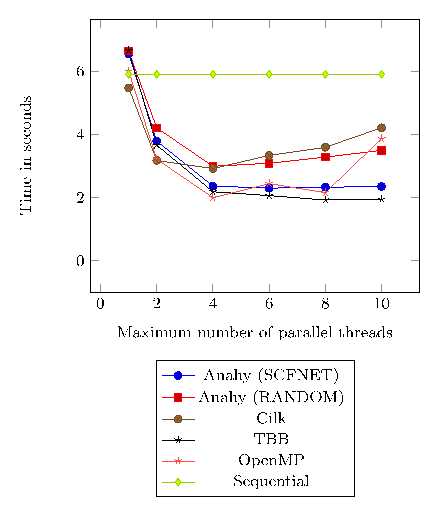
\includegraphics[width=0.44\textwidth,angle=0]{figs/sw_1000_10.eps}
	\caption{Execution of the Smith-Waterman algorithm, each thread calculatig a block of $10 \times 10$ elements.}
	\label{fig:SW}
\end{figure}

The Smith-Waterman is a dynamic algorithm conceived to align sequences of characters. In Figure~\ref{fig:SW} we present the results obtained matching one string of 1,000 characters against 1,000 strings of 1,000 characters each one. The alignment was achieved calculating blocks of $10 \times 10$ elements from the algorithm's work matrix in separate threads. In this graphic, we can observe that the better executions times were obtained when the maximum number of parallel threads was limited to four, except to TBB that in this experiment could exploit the hyper-threading. In this graph we highlight the difference of performance between the two curves representing two different heuristics to prioritize threads in Anahy: the implementation employing the SCFNET heuristic is clearly better than when the RANDOM one is employed. This fact indicates that the use of an elaborated scheduling strategy, taking into account the application requirements, could affect positively the final performance, regardless the overhead introduced by the scheduling operations.

% QUICKSORT

The second application tested was the Quicksort sorting algorithm. In our tests we took an array of 1,000,000 integer values, containing all the number in the interval $[0, 999,999]$, randomly shuffled. The method we used to parallelize the program was running each recursive call to Quicksort in a new thread. As the recursion of the algorithm can go very deep, thus generating threads with too little work to do, we used a threshold equal to 1,000, i.e., whenever the sorting method receives an array whose size is less than or equal to 1,000, it calls Selection sort, an iterative and stable sorting algorithm, without spawning any child threads. As we can see in Figure~\ref{fig:QS}, all tools achieved almost the same average execution time for all levels of parallelism in the X-axis. Also we could notice that for this instance of the problem running over Anahy, using RANDOM or SCFNET scheduling algorithm doesn't affect badly in the final performance, so the order of execution of threads doesn't affect the size of the scheduling in this case.

\begin{figure}

\begin{tikzpicture}
    \begin{axis}
    [
        x tick label style={
            /pgf/number format/1000 sep=},
        ylabel={Time in seconds},
        xlabel={Maximum number of parallel threads},
        enlargelimits=0.15,
        cycle list name=color2,
        legend style={at={(0.5,-0.25)}, anchor=north, font=\small, legend cell align=center},
        scale=0.9,
        ymin=0,
        xmin=1
    ]

\addplot
    coordinates { (1,0.6433586) (2,0.3243749) (4,0.1709939) (6,0.1511108) (8,0.1353574) (10,0.1373824) };
\addplot
    coordinates { (1,0.6379632) (2,0.3243135) (4,0.1695245) (6,0.1499195) (8,0.1351627) (10,0.136144) };
\addplot
    coordinates { (1,0.6379366) (2,0.3216966) (4,0.1699995) (6,0.1507495) (8,0.1363323) (10,0.1384655) };
\addplot
    coordinates { (1,0.6578617) (2,0.3319039) (4,0.1750612) (6,0.1547782) (8,0.1393562) (10,0.1412169) };
\addplot
    coordinates { (1,0.6568872) (2,0.3374134) (4,0.1843884) (6,0.1646282) (8,0.1443955) (10,0.20499) };
\legend{Anahy3 (RANDOM),Anahy3 (SCFNET),Cilk Plus,TBB,OpenMP}

    \end{axis}
\end{tikzpicture}
\caption{Executions of Quicksort for an array of size 1,000,000 and threshold equal to 1,000.}
\label{fig:QS}
\end{figure}

% MULTIPLICAÇÃO DE MATRIZES

The last application tested was a basic square matrix multiplication, like $A = B \times C$. The method we used to parallelize was creating a function to compute each line of $A$ in a separate thread. Inside this function, we create different threads to compute each column of that row concurrently. Using this method we have a DCG with two levels of ancestor threads, what scales well for the parallelism we are exploring here. In Figure~\ref{fig:MM} we show the results considering that all three matrixes have $500 \times 500$ cells. OpenMP achieves the smallest average times, while shows the worst scalability. When using SCFNET algorithm, Anahy shows results that are very close to the ones provided by Cilk Plus. However, using the RANDOM scheduling algorithm the execution times of Anahy and his scalability are negatively affected, so in this problem it's important to employ a scheduling algorithm that's aware of the graph structure. Though TBB doesn't show the best execution times, its scalability is the greatest among the tested tools, for this case.

\begin{figure}

% WRONG PLOT!!

\begin{tikzpicture}
    \begin{axis}
    [
        x tick label style={
            /pgf/number format/1000 sep=},
        ylabel={Time in seconds},
        xlabel={Maximum number of parallel threads},
        enlargelimits=0.15,
        cycle list name=color2,
        legend style={at={(0.5,-0.25)}, anchor=north, font=\small, legend cell align=center},
        scale=0.9,
        ymin=0,
        xmin=1
    ]

\addplot
    coordinates { (1,0.2998509) (2,0.1510404) (4,0.0788937) (6,0.0708814) (8,0.0624345) (10,0.0635974) };
\addplot
    coordinates { (1,0.3020884) (2,0.1508999) (4,0.0786585) (6,0.0689798) (8,0.0631871) (10,0.0633123) };
\addplot
    coordinates { (1,0.1163602) (2,0.0584618) (4,0.0307714) (6,0.0321002) (8,0.0329874) (10,0.0354671) };
\addplot
    coordinates { (1,0.3000244) (2,0.1508803) (4,0.0790323) (6,0.0736677) (8,0.0700784) (10,0.0715612) };
\addplot
    coordinates { (1,0.125397) (2,0.0642284) (4,0.0344015) (6,0.0412318) (8,0.0314295) (10,0.036624) };
\legend{Anahy3 (RANDOM),Anahy3 (SCFNET),Cilk Plus,TBB,OpenMP}

    \end{axis}
\end{tikzpicture}
\caption{Resuls from the multiplication of matrixes of size $500 \times 500$, being each cell of the resulting matrix computed concurrently.}
\label{fig:MM}
\end{figure}

In this section we have presented only a small part of the set of experiments achieved in the context of our research. Those results allow us to conclude that multithread environments can apply scheduling strategies based on pure list algorithms to improve the performance of the execution, achieving competitive levels compared to the main tools in the industry. We have shown also that different heuristics to prioritize threads can modify the final performance.

\section{Concluding Remarks}\label{sec:conclusion}

List scheduling algorithms are the basis for many scheduling techniques for various programming environments. In particular, Cilk and Athreads use this concept together with a heuristic to prioritize the execution of threads in the critical path to schedule threads dynamically at application level. In this kind of environment, the main challenge is to find the critical path of an application described in terms of a DCG instead of a DAG, as tipical list algorithms are used to deal with.

This work presented a strategy to build a DGC representing a multithreaded program apart from a DAG describing a dataflow program and a set of experiments to evaluate the impact of approximations of list scheduling strategies on an actual dynamic runtime environment. This allowed us to compare DAG schedules obtained in static scenarios with DCG schedules for dynamic executions, where both DAG and DCG represent the same program. It also presented a multithread scheduling strategy based in the Critical Path of the application. This strategy considers that the Critical Path will be present in the left most threads of a DCG. 

Performance results shown that the scheduling strategy applied to the DCGs can provide execution times as good as those provided by regular list scheduling applied to DAGs, when both describe the same application. The limits of list scheduling, when the distance to the Critical Path is the attribute priority of the tasks, were still preserved in the proposed scheduling strategy.

We conclude that list scheduling algorithms can be introduced in runtimes of multithreaded environments since good performances can be effectively achieved. The programmer must, nevertheless, be aware of the adopted scheduling strategy to organize the relationships among tasks and hence harvest the benefits of its characteristics.

\bibliographystyle{spmpsci}
\bibliography{bibs}

\end{document}

% BibTeX users please use one of
%\bibliographystyle{spbasic}      % basic style, author-year citations
%\bibliographystyle{spmpsci}      % mathematics and physical sciences
%\bibliographystyle{spphys}       % APS-like style for physics
%\bibliography{}   % name your BibTeX data base

